%\documentclass{article}
\documentclass[titlepage,12pt,a4paper]{article}
\usepackage[utf8]{inputenc}
\usepackage{parskip}
%\usepackage[T1]{fontenc}
%\usepackage[ngerman]{babel}
\usepackage{amsmath}
%\usepackage{enumitem}
\usepackage{graphicx}
%\usepackage[numbers]{natbib}
%\usepackage{authblk}
%\usepackage{titlepic}
%\usepackage{amsfonts}
%\usepackage[usenames,dvipsnames,svgnames,table]{xcolor}
\usepackage{listings, color}
\usepackage{url}
\usepackage{hyperref}
\usepackage{subfig}

\let\stdsection\section
\renewcommand\section{\newpage\stdsection}

\title{Memory Hacking Discoveries\\in The Wind Waker}
\author{Christopher Serr, Sergey Papushin}

\begin{document}

\maketitle

%\begin{abstract}
%\end{abstract}

\tableofcontents
\clearpage

\section{Superswimming}
Superswimming allows the player to travel huge distances through the ocean of The Wind Waker. This is done by turning Link around rapidly while he is in the water. Every time he turns around, he'll accelerate a bit and will get faster and faster over time, eventually reaching extremely fast speeds. The game's air meter only lasts 30 seconds, so it's important to choose the right moment to stop charging the Superswim and release it. Charging too long will cause Link to drown before he comes to a stop, and vice versa. In order to maximize distance, a Superswim should be released after around $\frac{2}{3}$ of the total time that Link can be in the water before drowning. This means that the optimal release time is after around 20 seconds for most Superswims, but refilling the air meter during a Superswim by getting close to a shore will increase the total time, resulting in a later distance-maximizing release time.

\begin{figure}[!htb]
	\centering
	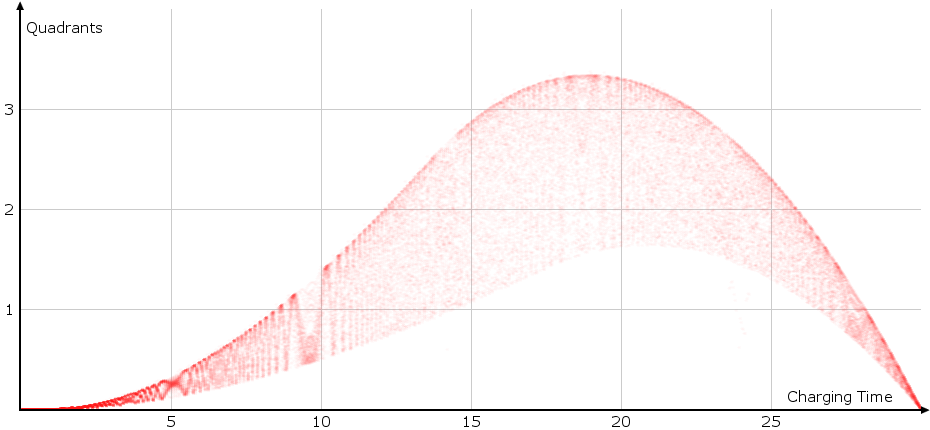
\includegraphics[width=\textwidth]{SSDistance}
	\caption{Range of distances possible based on when the player releases the Superswim}
	\label{fig:SSDistance}
\end{figure}

Figure \ref{fig:SSDistance} shows the range of distances that the player can get after releasing the Superswim. Notice how the graph varies greatly, even if looking at a specific point in time. This is because the way that Link enters the water and how he interacts with the waves slightly affects the progression of the Superswim. However, this only slightly affects the overall trend in Superswim speed. 

\begin{figure}[htp]
	\subfloat{
      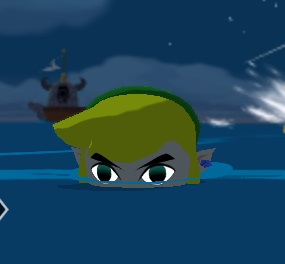
\includegraphics[width=0.175\textwidth]{SSFrame1}
    }
    \hfill
    \subfloat{
      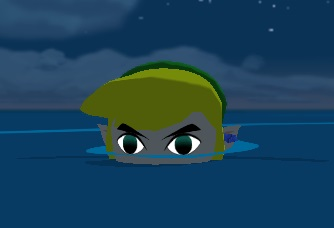
\includegraphics[width=0.175\textwidth]{SSFrame2}
    }
    \hfill
    \subfloat{
      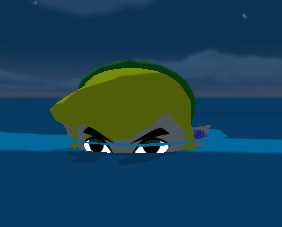
\includegraphics[width=0.175\textwidth]{SSFrame3}
    }
    \hfill
    \subfloat{
      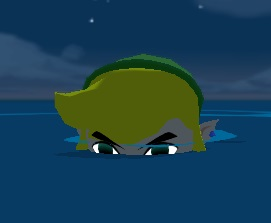
\includegraphics[width=0.175\textwidth]{SSFrame4}
    }
    \hfill
    \subfloat{
      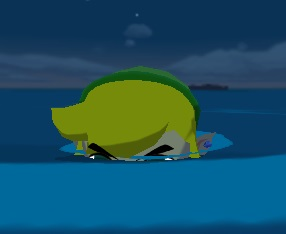
\includegraphics[width=0.175\textwidth]{SSFrame5}
    }
    \caption{Link cycling through his swimming animation}
    \label{fig:SSFrames}
\end{figure}

The most important thing to understand is that Link constantly cycles through his swimming animation. This swimming animation is shown in Figure \ref{fig:SSFrames}. Although the speed of the Superswim will generally increase while charging, the exact speed is also directly affected by where Link is in his animation cycle. This speed is actually determined 2 frames after he turns around for the last time after releasing the Superswim. All of this is made more complicated, however, by the fact that the rate at which Link's swimming animation speed plays depends on Link's speed, meaning that the faster Link gets, the faster his animation is played. Aliasing will also come into play, though. While the animation cycle lasts a few seconds when Link is slow, the entire animation will take less than a frame when Link is fast enough. Since the game runs at 30 frames per second, the swimming animation can only be sampled 30 times per second, so the game isn't able to accurately play the animation when it takes less than 1 frame. Once the animation's period is exactly 1 frame, it'll look like it completely comes to a stop, since the game will always sample the same part of the animation. Once it's faster than a single frame, it'll  look like it's going backwards until it takes half a frame to complete, when it yet again comes to a stop.  

\begin{figure}[!htb]
	\centering
	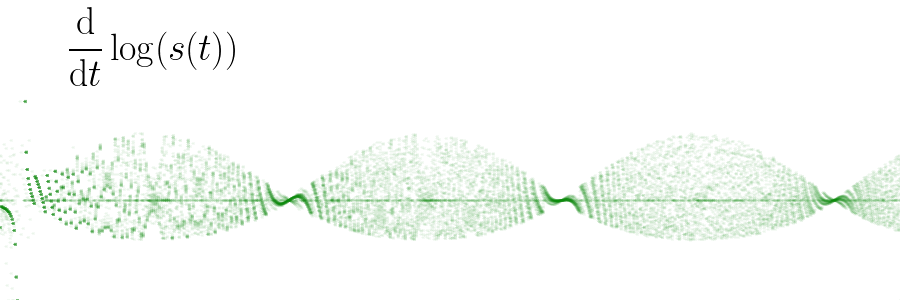
\includegraphics[width=\textwidth]{SSDerivative}
	\caption{Logarithmic derivative of the speed function over time}
	\label{fig:SSDerivative}
\end{figure}

This behaviour can be seen in Figure \ref{fig:SSDerivative}. This graph visualizes the relative change in speed per frame, which is directly related to Link's sampled animation speed. The speed change is exactly zero whenever his animation appears to stop, which is when it takes exactly $1, \frac{1}{2}, \frac{1}{4}, \frac{1}{8}, \ldots, \frac{1}{2^n}$ frames. Also, the faster that the animation speed appears to be, the more Link's speed also changes. The period of this function is about 9.5 seconds, so after around $9.5, 18, 27.5, \ldots, 9.5 n$ seconds, Link's animation will appear to come to a stop, and Link's speed will no longer change. This is really useful, since 18 seconds is also around the time that a Superswim's distance can be maximized.

A good strategy is to release while Link's animation is being played slowly. This is because it's easier to predict what the speed will be 2 frames after the Superswim is released based on what is displayed when pausing right before releasing. This is mostly due to there being less variation in the animation speed while it is played slowly.

\section{Event System}
The Wind Waker uses an event system in order to start and stop cutscenes. This event system ensures that you will never gain control of Link during a cutscene, and that you will regain control once the cutscene is over. However, one of the biggest glitches in The Wind Waker, storage, involves a desync of the Event System, allowing you to pause or cancel many cutscenes. The Wind Waker's event system uses several variables in order to maintain events.

\subsection{Event System Variables}
The Wind Waker's event system uses several variables in order to maintain events.
	
\subsubsection{Event State}
This variable represents your current event state.
\begin{itemize}
	\item 0: Normal state. This means that you're not in an event. This usually control of Link with the GUI on the screen.
	\item 1: Talking to an NPC. Talking to KoRL or a mailbox are examples of this state.
	\item 2: In a cutscene. This includes cutscenes like the CS before Helmaroc or receiving the Delivery Bag.
	\item 3: Link-only cutscene. Pulling out the Wind Waker, pulling out the Sail, or drinking Soup are all examples.
\end{itemize}

\subsubsection{Start Event}
When this variable is set to 1, this tells the game to start the event that is loaded into memory. When this is done, this variable gets reset to 0.

\subsubsection{Stop Event}
When this variable is set to 1, this tells the game to stop the current event. When this is done, this variable gets reset to 0. The state when "Stop Event" is set to 1 while the Event State is normal is commonly known as storage.

\subsubsection{Event Memory}
This variable is used as a place to store event data in the memory. This is done before an event is started.

\subsection{Common Event Sequences}
Events normally follow a set sequence. The game loads an event into the memory, starts the event, sets the Event State properly, executes the event, stops it, and then resets the Event State so that you regain control of Link.

\subsubsection{Normal sequence for an event}
\begin{enumerate}
	\item Event is loaded into Event Memory, Start Event is set to 1
	\item Event is executed, Event State is set, Start Event is reset to 0
	\item Stop Event is set to 1
	\item Event State is reset to 0, event is stopped, Stop Event is reset to 0
\end{enumerate}

Normally, when playing the Wind Waker, both camera lock and Wind Waker playing get cancelled when pressing B. If you hit the ground 3 frames after pressing the B button, Camera Lock gets cancelled but the Wind Waker playing does not get cancelled properly. When the event is finally stopped properly by pressing the B button again, Stop Event is set to 1 again but never reset to 0 because the Event State is already 0. This is the most common way to obtain storage.

\subsubsection{Storage sequence}
\begin{enumerate}
	\item Wind Waker button pressed, event is loaded into Event Memory, Start Event is set to 1
	\item Event State is set to 3, event is executed, Start Event is reset to 0
	\item B button is pressed on correct frame, Stop Event is set to 1, Camera Lock part of event gets cancelled
	\item Event State is set to 0, Stop Event is reset to 0
	\item B button is pressed again, Stop Event is set to 1, Wind Waker playing part of event gets cancelled
\end{enumerate}

\subsection{Do Events Actually Get Stored?}
Surprisingly, although the glitch is called storage, events never really get stored. Although we see some event data get stored in the Event Memory, this memory is only used by the event that is currently being started and not really involved with storage.

Instead of being stored, events are usually paused or cancelled when trying to start them while having storage active. Some events, like the cutscene in the main room of DRC, get completely cancelled. Others, such as talking to KoRL, will resume whenever another event starts, such as pulling out the Wind Waker. In general, the only thing that we really see getting stored is the Stop Event being set to 1 despite regaining control of Link, so in some ways, the name “storage” is still fitting.

\section{Collision Detection}
A common use of storage is with chests and doors, as normally starting these events will temporarily change Link’s collision detection. In general, each actor has a state that tells the game how precise the physics need to be. This contains multiple flags that turn individual parts of the physics calculation on or off. There are also two levels of "precision" for collision detection. The game first checks for a Rough Collision (if active), and only if the rough calculation detects a collision, will the game check for a Precise Collision (if active). 

\textbf{Chest Storage:} Rough Collision is on, Precise Collision is off\\
\textbf{Door Cancel:} Rough Collision is off, Precise Collision is off

\subsection{Collision Detection Flags}
There are also other flags that can turn off the collision detection for an actor completely. This will cause Link to fall through everything. Even loading zones don’t work anymore because they rely on collision detection.

The physics system will also write information for other systems in the game to use. For example, the physics system will activate the "At Wall" flag when Link is standing next to a wall so that the rest of the game knows if Link can start to sidle.

These are the flags in the "physics state" that we have figured out so far:
\begin{itemize}
	\item At Shore
	\item No Wall Collision (Door Cancel)
	\item No Climbing
	\item No Ground Collision
	\item No Collision
	\item No Precise Collision (Chest Storage)
	\item At Wall
	\item On Ground
\end{itemize}

\section{Warp System}
The Wind Waker uses the Warp System whenever the game needs to switch between stages or start major cutscenes in these stages. The Warp System consists of exits, which send Link to a different stage, and spawns, which is where Link appears in the new stage. Exits and spawns interact during transitions between two different stages.

\subsection{Exits}
In The Wind Waker, exits are basically the start to a warp, and usually are either loading zones or triggers for major cutscenes. Exits set certain variables of the warp system and then initiate a warp in order to send Link to a different stage.

\subsubsection{Stage}
A stage is a separate area in the game, sometimes also consisting of multiple rooms. Traveling between stages requires the use of a warp. The exit changes the destination stage so that the proper stage can load. Some examples of stages are: 
\begin{itemize}
	\item All of Beedle’s ships (Obshop)
	\item Pirate Ship (PShip)
	\item Hyrule Exterior (Hyrule)
	\item Great Sea (sea)
	\item Link’s house (LinkRM)
\end{itemize}

\subsubsection{Room ID}
A room is an area within a stage. Many stages consist of only one room, but some stages, such as dungeons or the Great Sea, contain many different rooms. Exits set a Room ID so that Link can be placed in the correct room within a stage.

\subsubsection{Spawn ID}
The Spawn ID defines which spawn the game should choose to place Link at within the room. Each spawn has specific properties that define how Link will spawn in the new stage.

\subsubsection{Layer Override}
Rooms often have layers, each of which can contain actors and triggers. The Layer Override determines which one of these layers the game should load. Loading zones always set the Layer Override to -1, which forces the room to use flags and logic defined by the stage in order to determine which layer to use. Events, however, usually use the Layer Override so that the room loads the proper actors required for the event.

\subsubsection{Is Warping}
When this variable is set to 1, the game begins the warping sequence and then uses the other variables (Stage, Room ID, Spawn ID, Layer Override) in order to load the correct new stage and use the correct spawn.

\subsection{Spawns}
Spawns are used in order to position Link within the newly loaded room. A spawn can also start an event if the event is part of the EVNT section in the stage header. Out of all all events supported by the stage, this section defines a subset with events which can be referenced by spawns. Each spawn has certain defined properties.

\subsubsection{Spawn ID}
Each spawn has a specific ID. The game chooses a spawn by matching the Spawn ID of a spawn with the one defined by the last exit.

\subsubsection{Spawn Position}
The spawn position, stored as X, Y, and Z coordinates, defines where Link will be placed in the new room.

\subsubsection{Event ID}
Most spawns have an Event ID of -1, which tells the game that it does not need to play an event. Some spawns, though, use an Event ID of 0 or greater, which tells the game to play a specific event defined in the stage. As a result, many cutscenes can only be played by spawning at a specific spawn.

\subsection{Special Exits}
Some exits set a Spawn ID of less than 0, which causes the spawn to be treated slightly differently.

\subsubsection{Voiding Out}
Whenever you void out, a Spawn ID of -1 is set, which tells the game to use the coordinates of your last spawn instead of choosing a spawn based on the Spawn ID.

\subsubsection{Beedle’s Ship}
When you enter Beedle’s Ship, the game stores the Room ID of the island that you entered Beedle’s Ship on, since the same Beedle room can be shared by multiple different islands. When exiting Beedle, the game sets the Room ID to the stored value and sets the Spawn ID to -2, indicating the exit on Beedle’s Ship.

\subsubsection{Spawn Point Not Found}
If the game can't find the spawn point provided to it by the exit, it sets the Spawn ID to -3.

\end{document}
